\begin{frame}[t]{Приставка  для единиц измерения \\ количества информации/данных: проблема}
\begin{columns}
	\begin{column}{5cm}
	\begin{center}
		Linux Ubuntu 14\\
		\vskip 0.2cm
		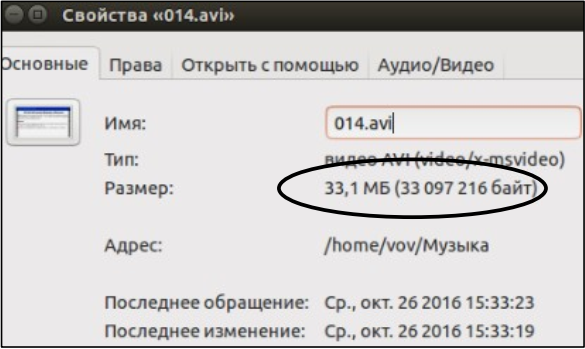
\includegraphics[scale=0.4]{ubuntu}
	\end{center}
	\end{column}
	\begin{column}{5cm}
	\begin{center}
		Microsoft Windows 7\\
		\vskip 0.2cm
		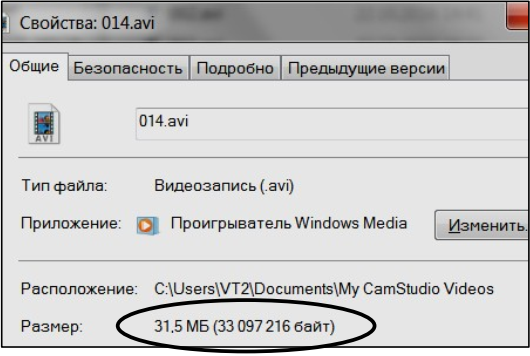
\includegraphics[scale=0.4]{windows}
	\end{center}
	\end{column}
\end{columns}
\begin{center}
	33 097 216 байт --- это \textbf{33,1}\color{black} МБ или \textbf{31,5} \color{black} МБ?
\end{center}
\end{frame}